\par Family tables are something that our team has discovered. They allow the user of the CAD program to create a generic model, which can then be customized to fit any situation. 
\par In CREO, this is done by clicking on "Tools", followed by "Family Tables", as shown in \ref{fig:Step1}. Then, the pop-up shown in \ref{fig:Step2} will appear. Pressing the button that the dark red arrow is pointing in \ref{fig:master} to will cause a new column to form, and pressing the button the bright red arrow is pointing to will cause a new row to form. 
\par Each row controls which instance of the model is affected, as identified by the black arrow and the grey arrows \ref{fig:master1}, while each column controls various aspects of each instance, as signified by the orange arrow, yellow arrow, and the green arrow in \ref{fig:master1}. The generic model is shown by the black arrow, and the children models by the grey arrows. 
\par In the column that the green arrow is pointing to in \ref{fig:master1}, the presence of a feature is affected, in this case the extrusion on the example model. 
\par What each column does is controlled by this pop-up, shown in \ref{fig:Step4}, which appears when "Create Column" is pressed. The light blue arrow points to where you can change what type of aspect is changed. Feature, identified by the dark blue arrow, allows control of the existence of a feature, dimension allows control of lengths. Dimension, shown by the purple arrow, allows us to control the value of a dimension in each model. This allows us to create different children models from a single generic model. There is an example of this in \ref{fig:Dim_Exa_1}, \ref{fig:Dim_Exa_2}, and \ref{fig:Dim_Exa_3}. 
\par For example, shown in \ref{fig:master1}, in the column identified by the brown arrow and the row identified by the lime arrow, a Y is displayed. While it is an Y, there will be that feature in that instance of the model. In same column, but the row identified by lavender arrow , the same Y is now a N. This has made the feature disappear in the model.All of this allows us to create three different models, one generic and two children, allowing us a great degree of flexibility in CAD. The three models can be seen in \ref{fig:Mod_Ins_1},\ref{fig:Mod_Ins_2}, and \ref{fig:Mod_Ins_3}.
% what each column does. 
\par You can see examples of this in our L pieces and our T pieces. All the L and T pieces are all created from a single generic model. We use a family table to change whether a both sides of the model are extruded, as well as whether there are axle or bearing holes. This allows us to create eight different specific models from a single model. For more information, see "Design Moto G4 Phone Case and T and L pieces" meeting. 
% Include page number. 

\begin{figure}[ht!]
\centering
  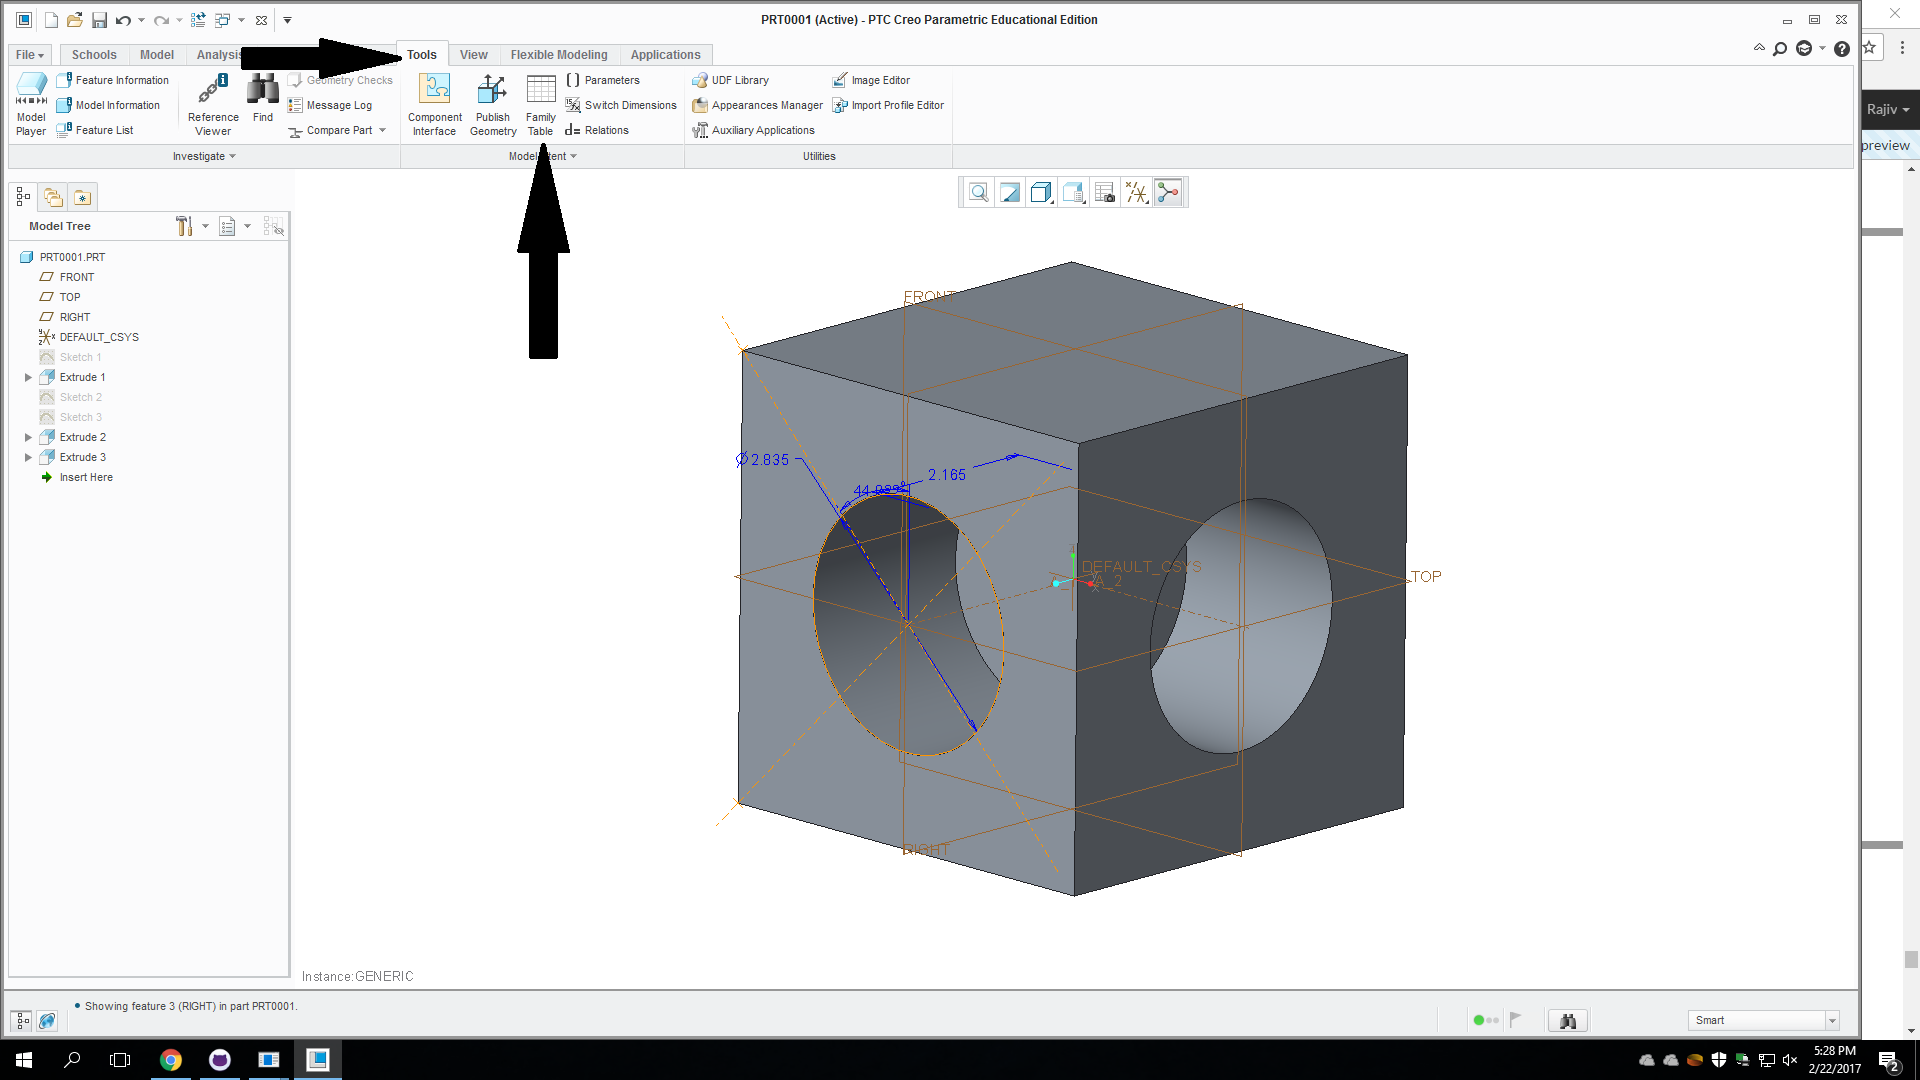
\includegraphics[width=0.7\linewidth]{CAD/Technique/FamilyTableFolder/Capture1_1.png}
  \caption{Opening a Family Table.}
  \label{fig:Step1}
\end{figure}

\begin{figure}[ht!]
\centering
  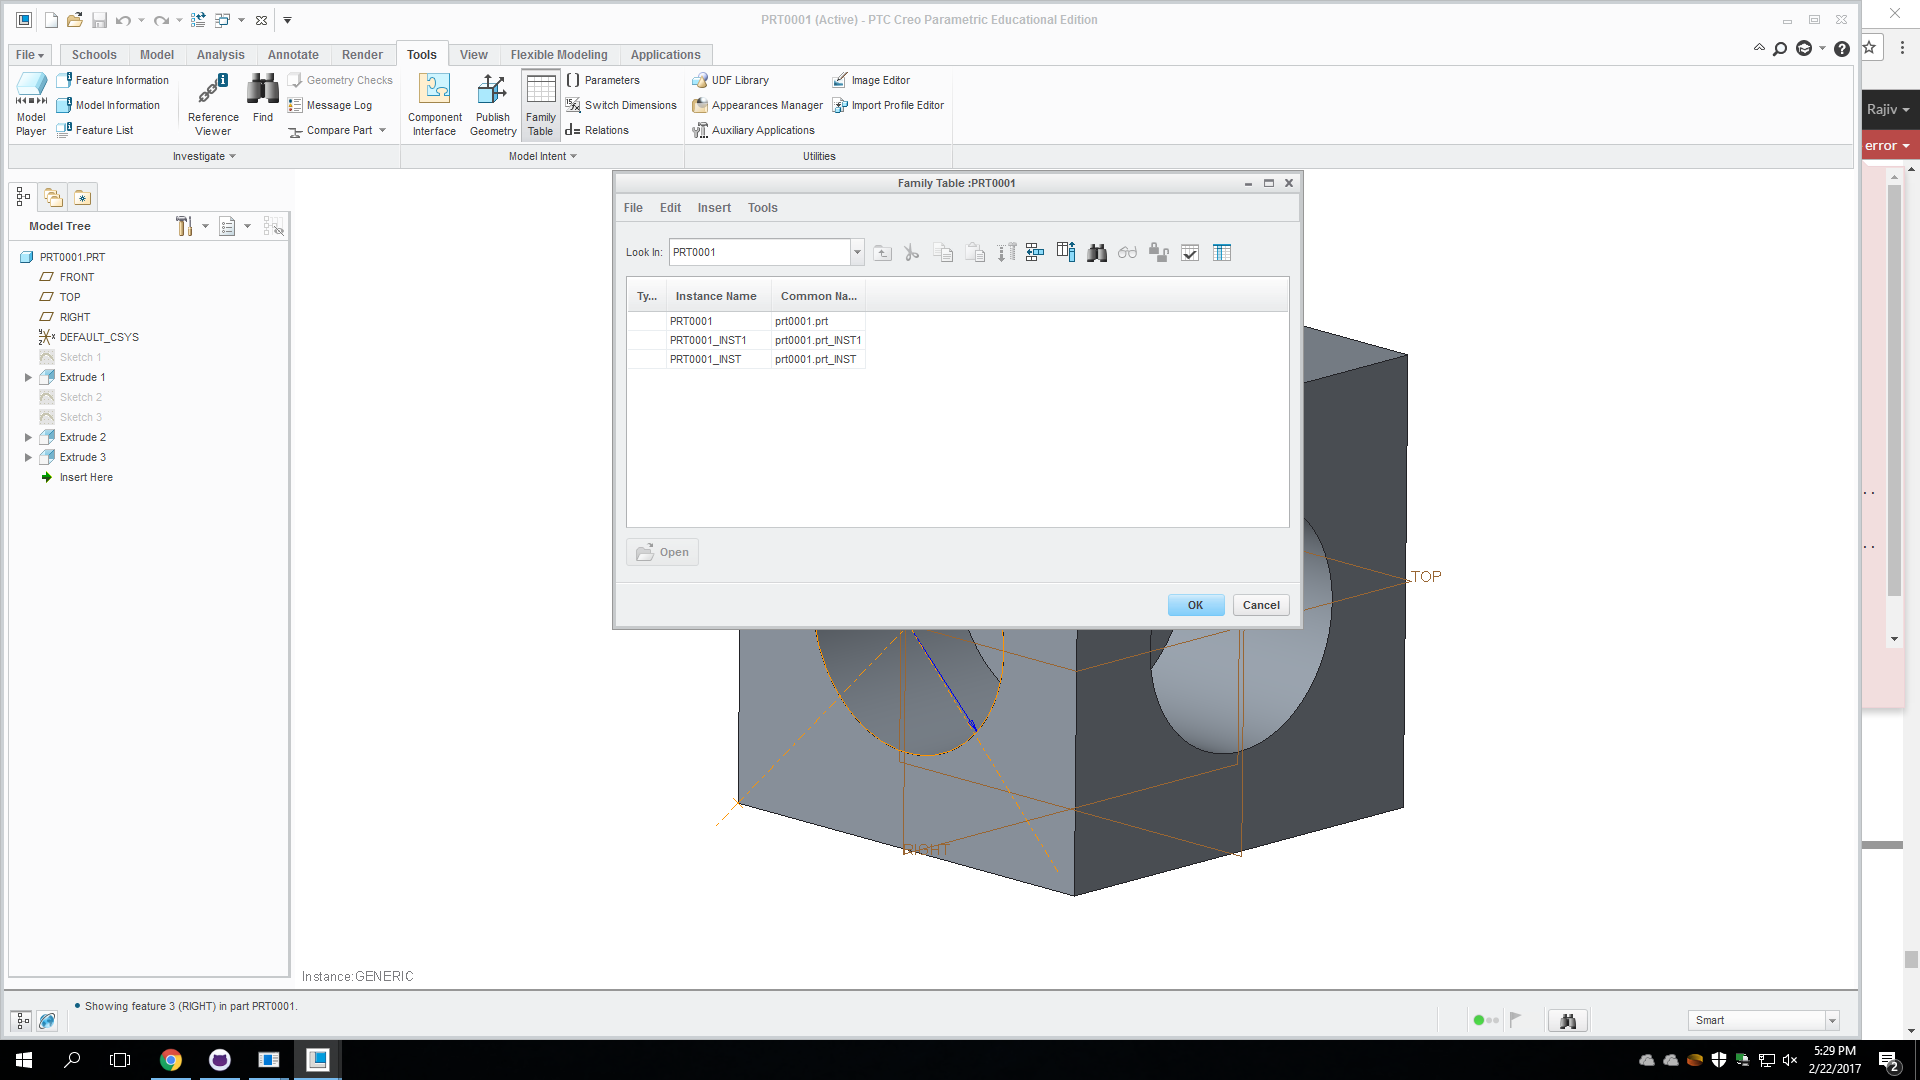
\includegraphics[width=0.7\linewidth]{CAD/Technique/FamilyTableFolder/Capture2.png}
  \caption{The Family Table Window.}
  \label{fig:Step2}
\end{figure}

\begin{figure}[ht!]
\centering
  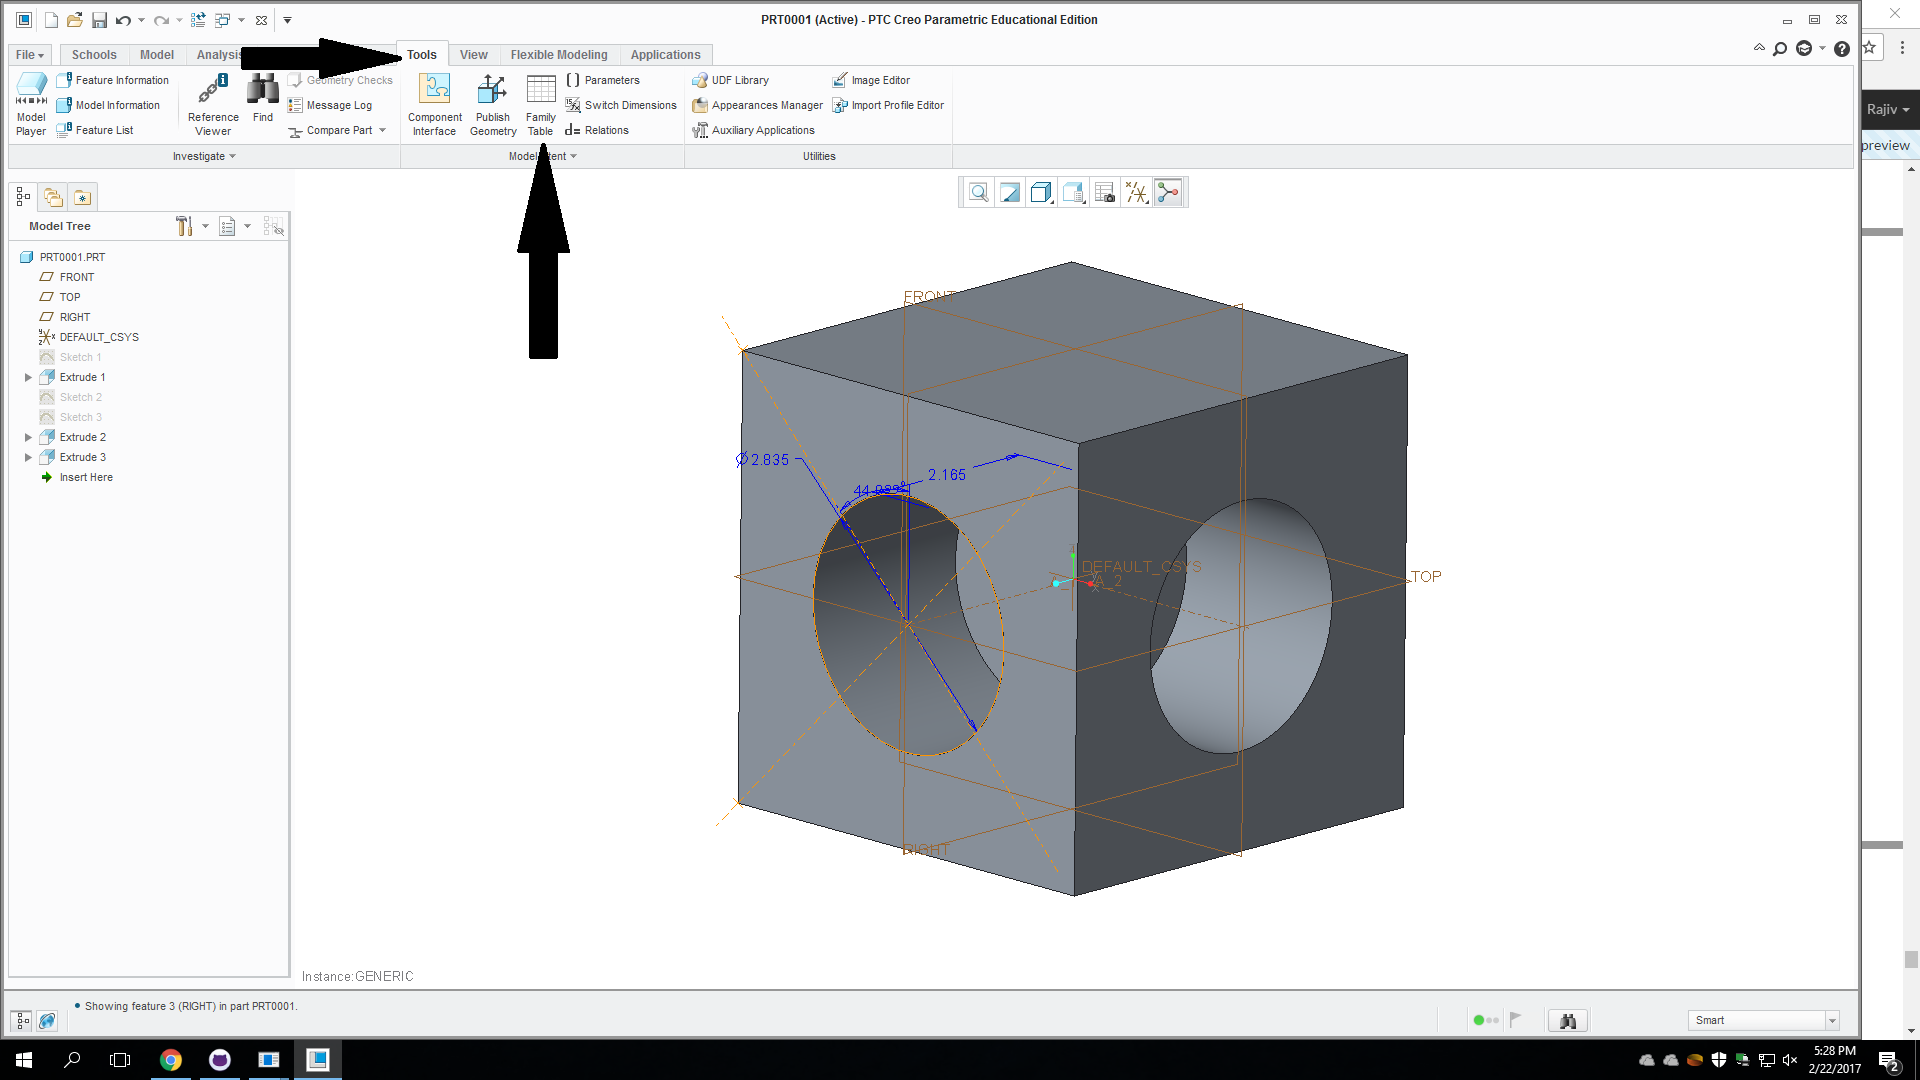
\includegraphics[width=0.7\linewidth]{CAD/Technique/FamilyTableFolder/Capture1_1.png}
  \caption{An explanation of what the family table window does.}
  \label{fig:master1}
\end{figure}
  
\begin{figure}[ht!]
\centering
  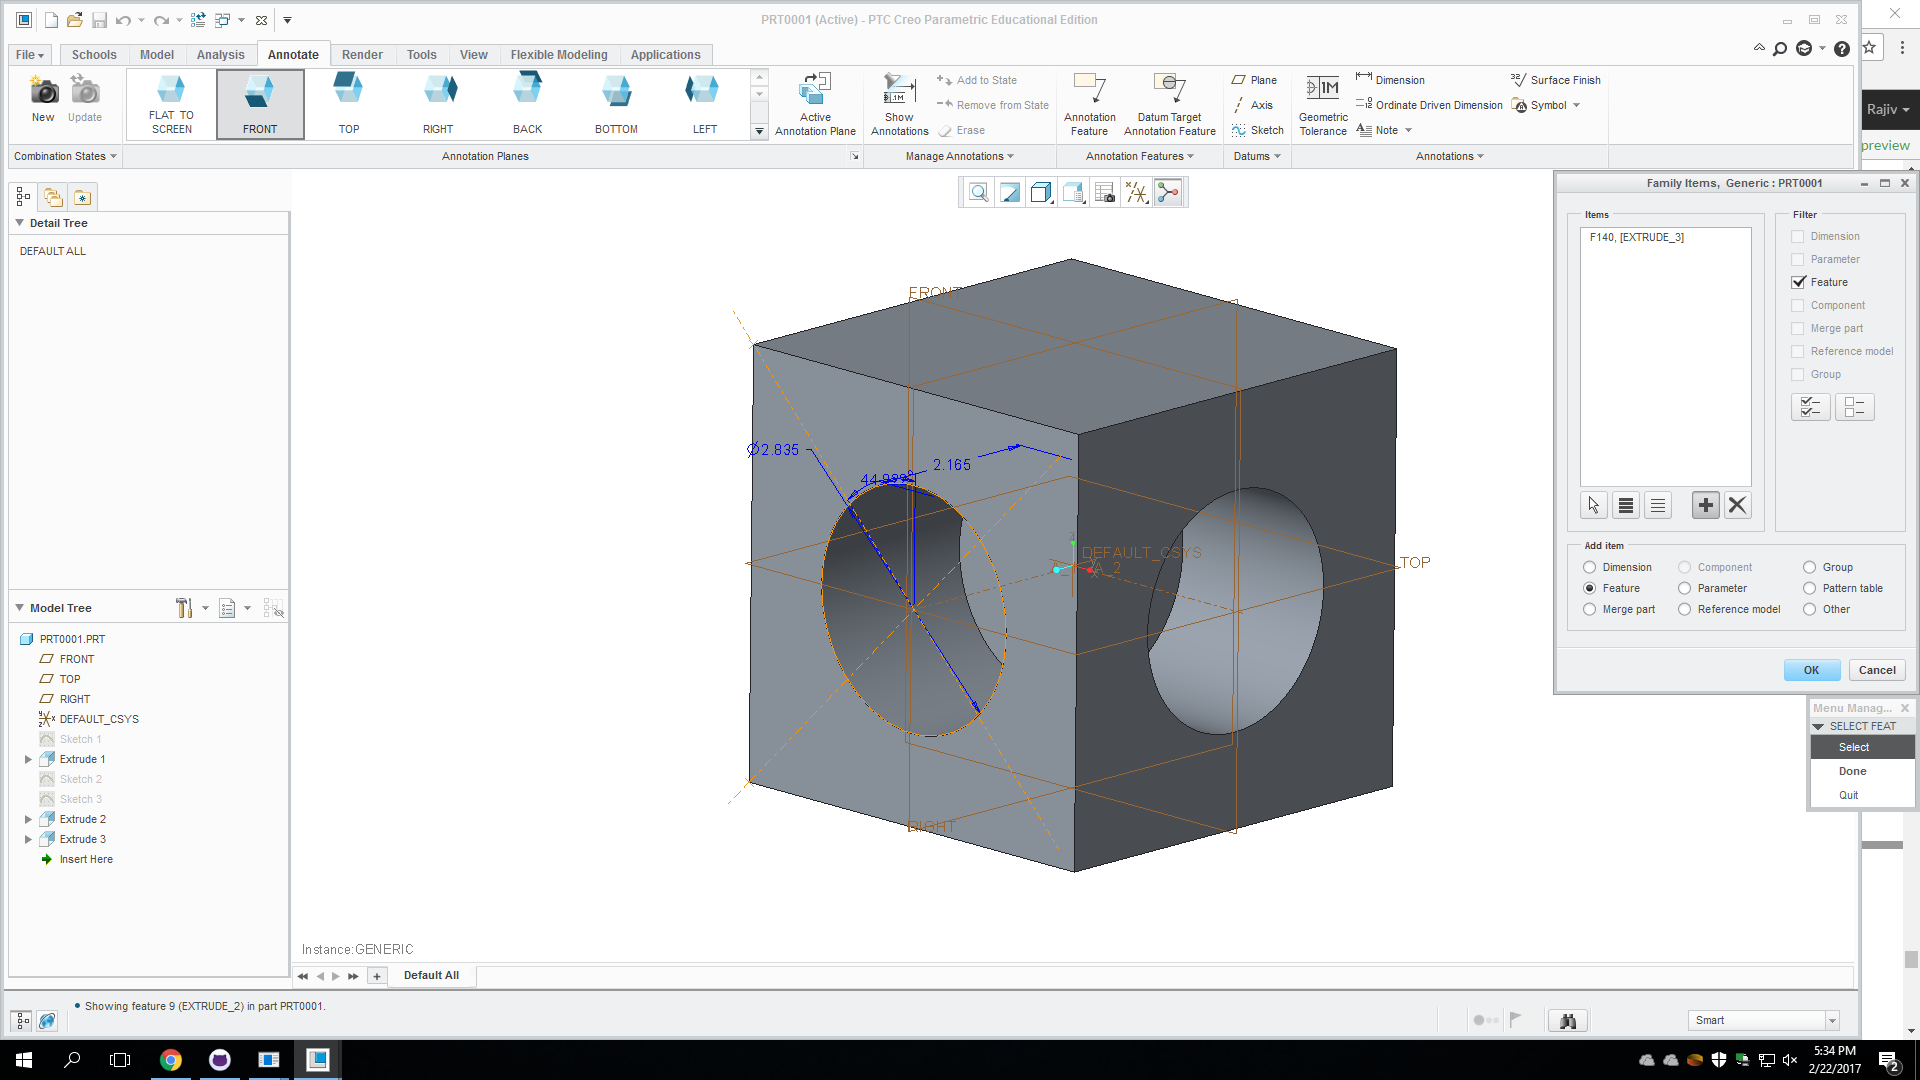
\includegraphics[width=0.7\linewidth]{CAD/Technique/FamilyTableFolder/Capture8.png}
  \caption{Settings customization window.}
  \label{fig:Step4}
\end{figure}
  
\begin{figure}[ht!]
\centering
  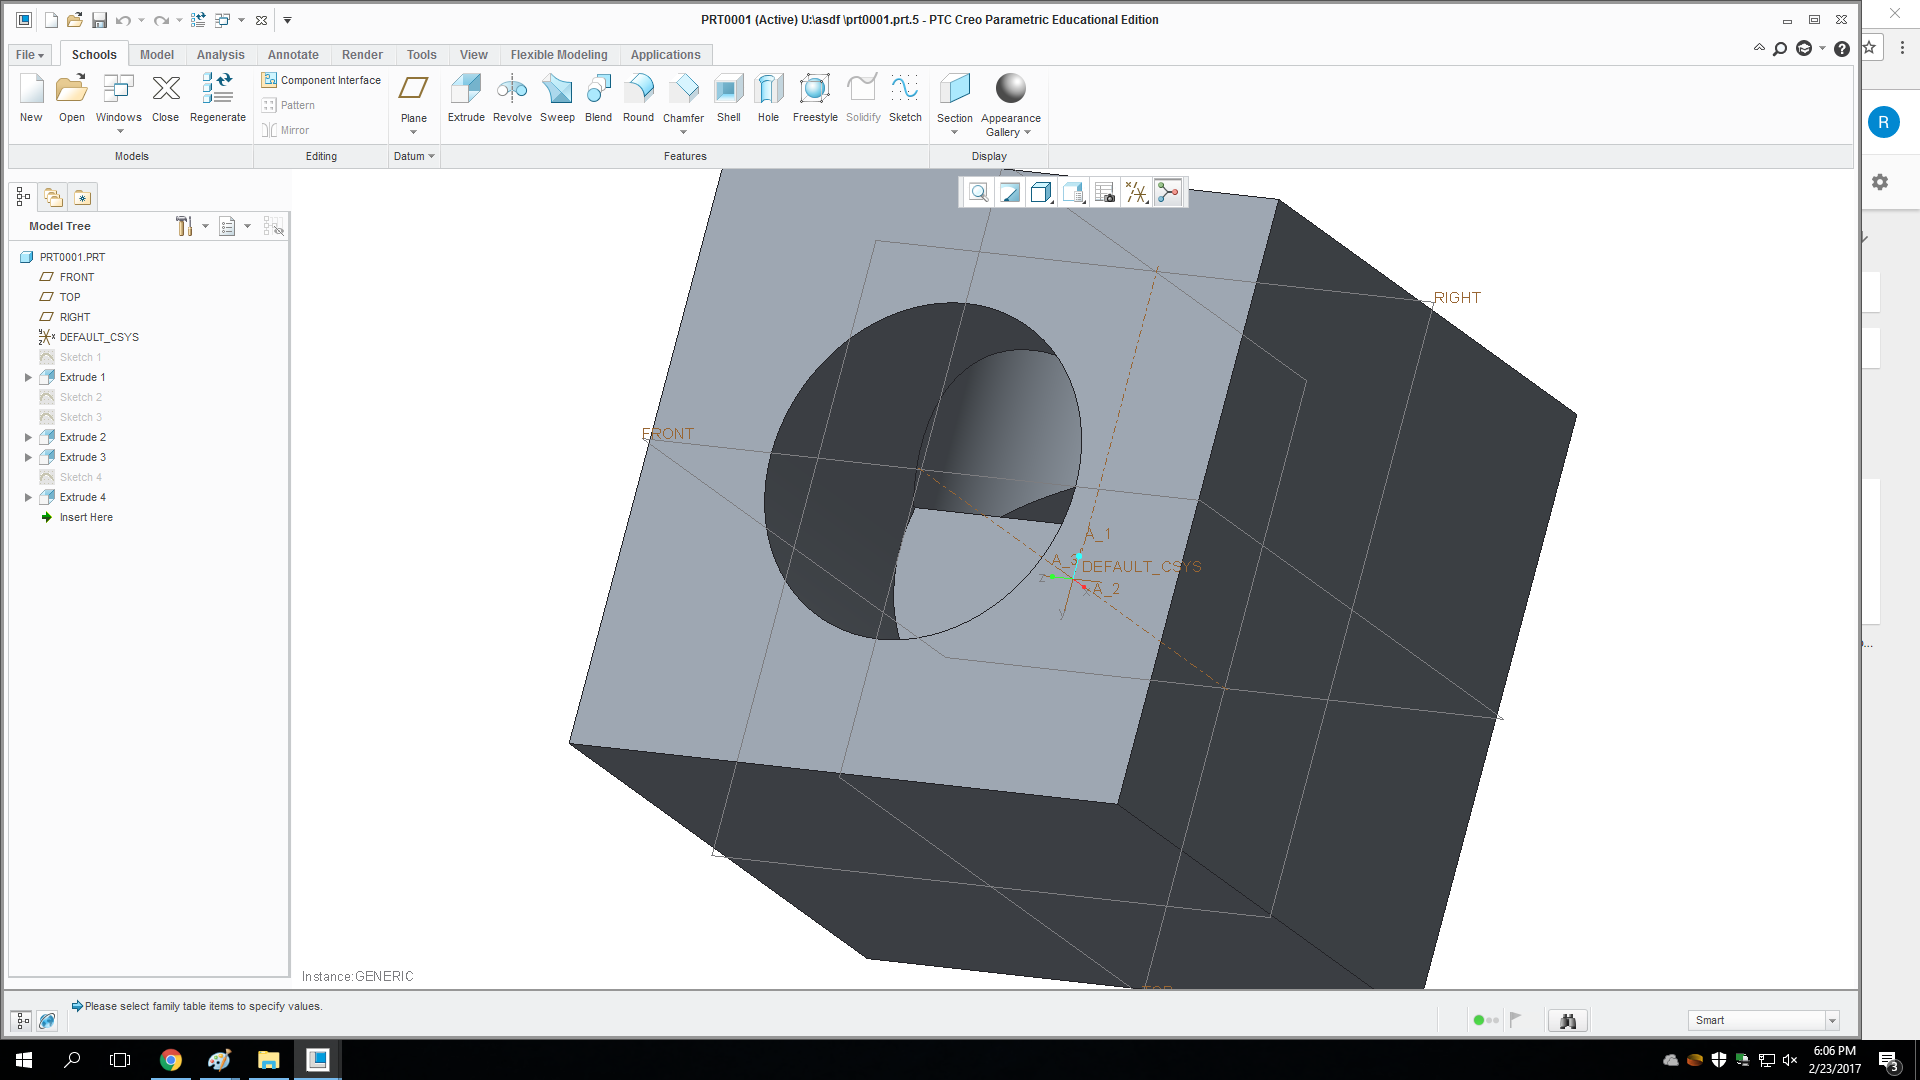
\includegraphics[width=0.7\linewidth]{CAD/Technique/FamilyTableFolder/Capture_1.png}
  \caption{Settings customization window.}
  \label{fig:Dim_Exa_1}
\end{figure}

\begin{figure}[ht!]
\centering
  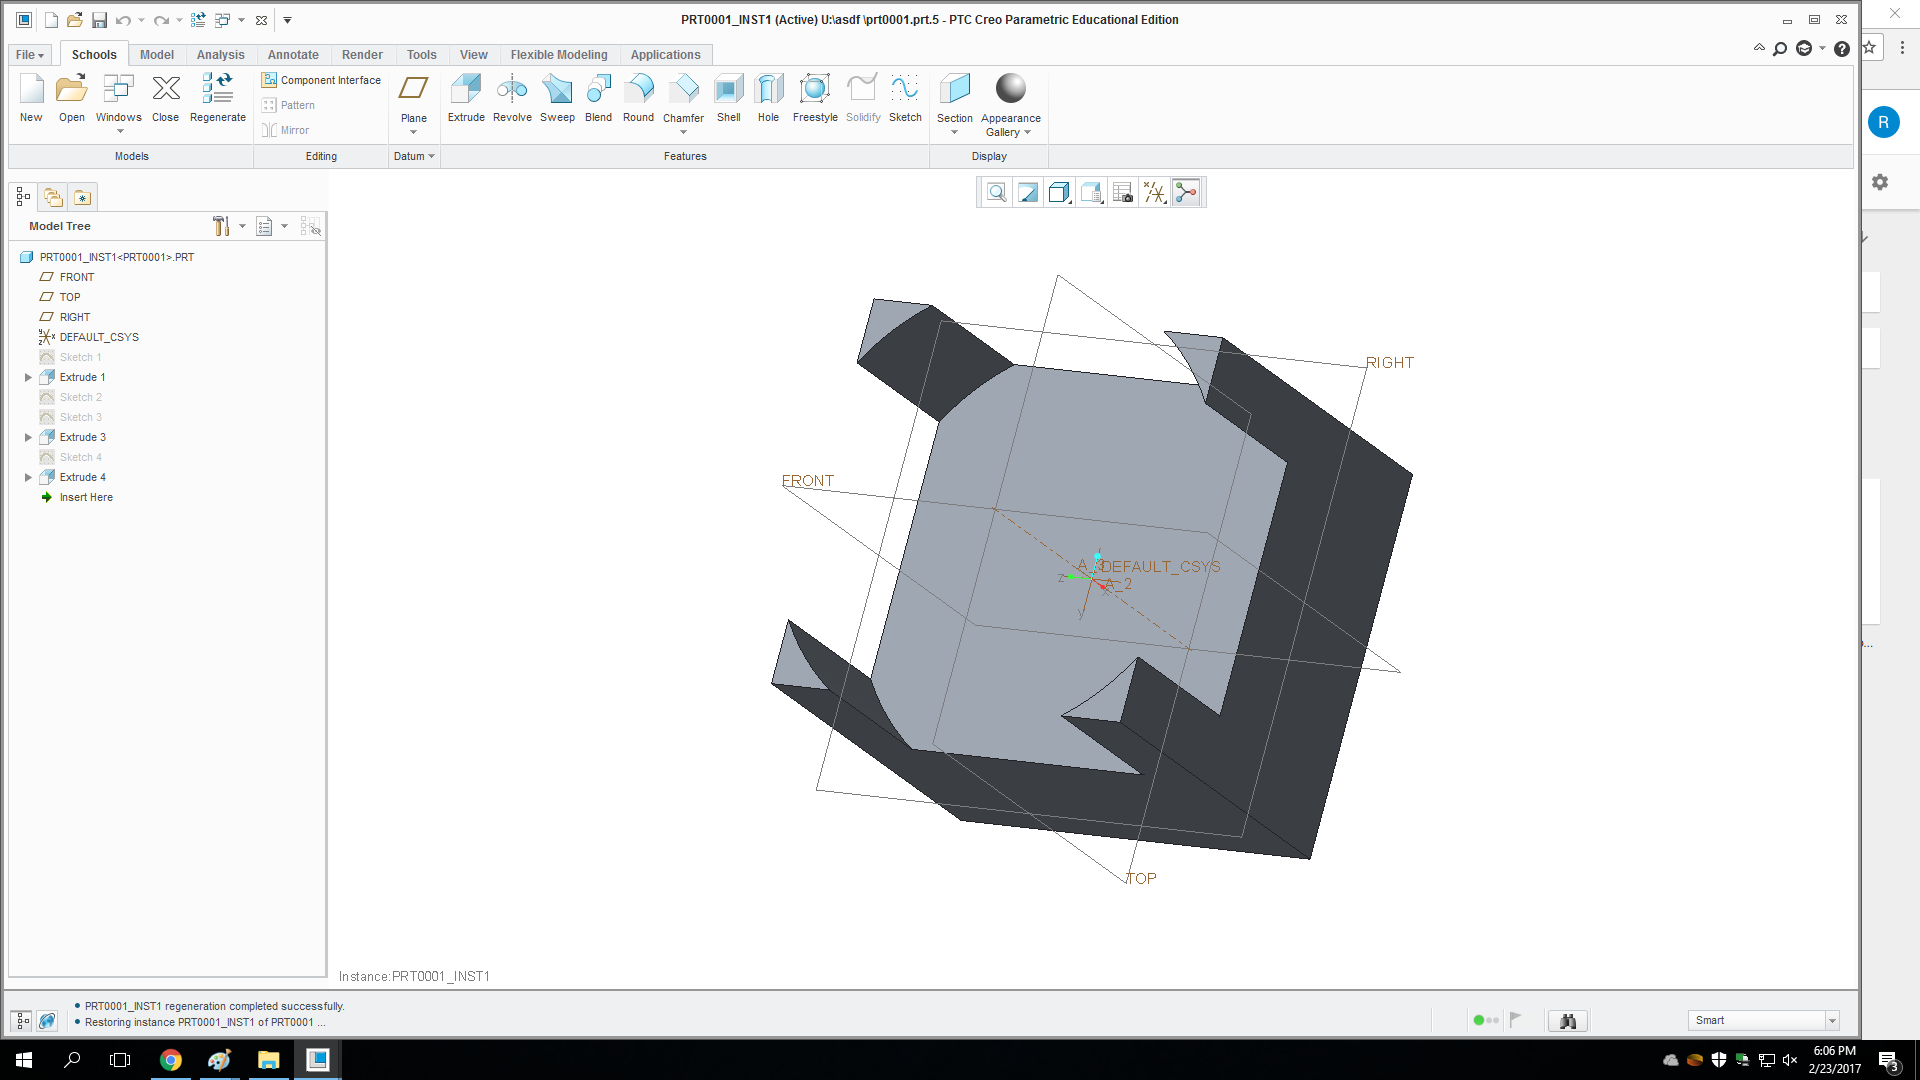
\includegraphics[width=0.7\linewidth]{CAD/Technique/FamilyTableFolder/Capture_2.png}
  \caption{Settings customization window.}
  \label{fig:Dim_Exa_2}
\end{figure}

\begin{figure}[ht!]
\centering
  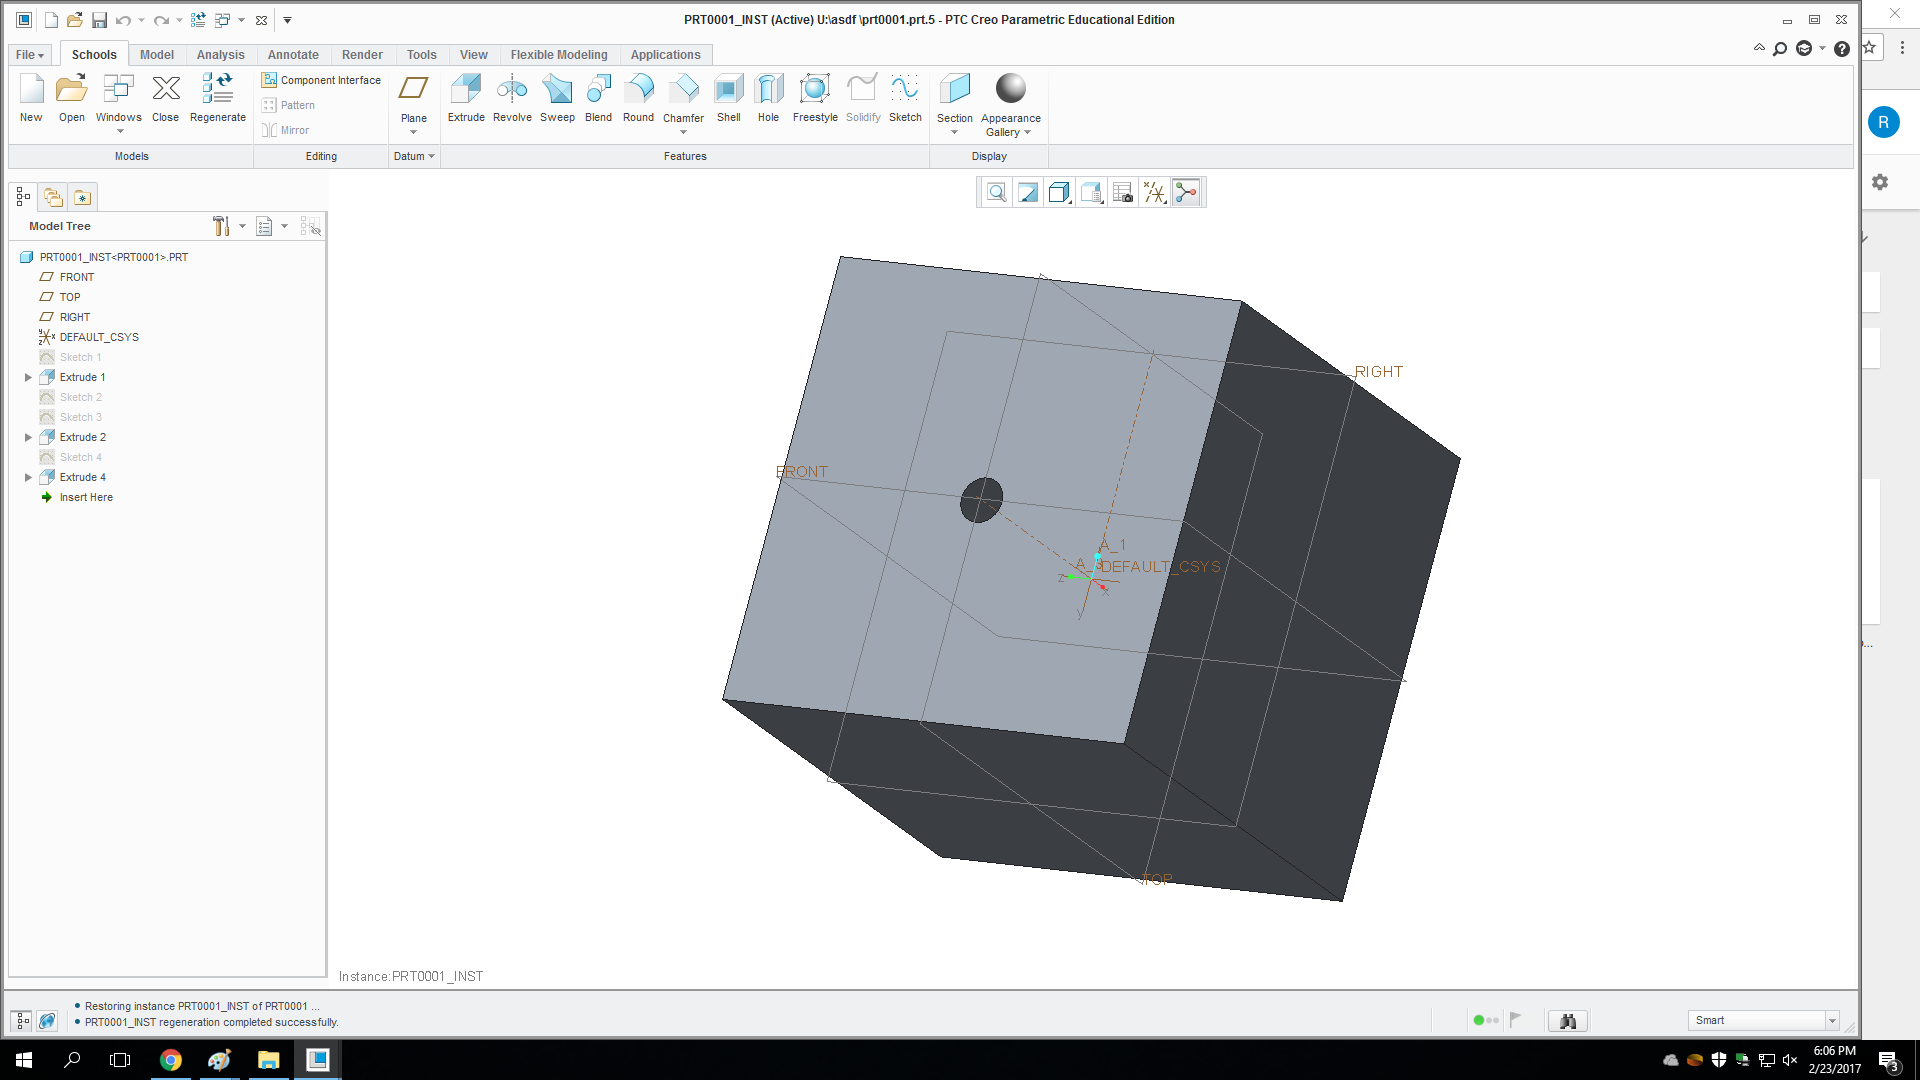
\includegraphics[width=0.7\linewidth]{CAD/Technique/FamilyTableFolder/Capture_3.png}
  \caption{Settings customization window.}
  \label{fig:Dim_Exa_3}
\end{figure}

\begin{figure}[ht!]
\centering
  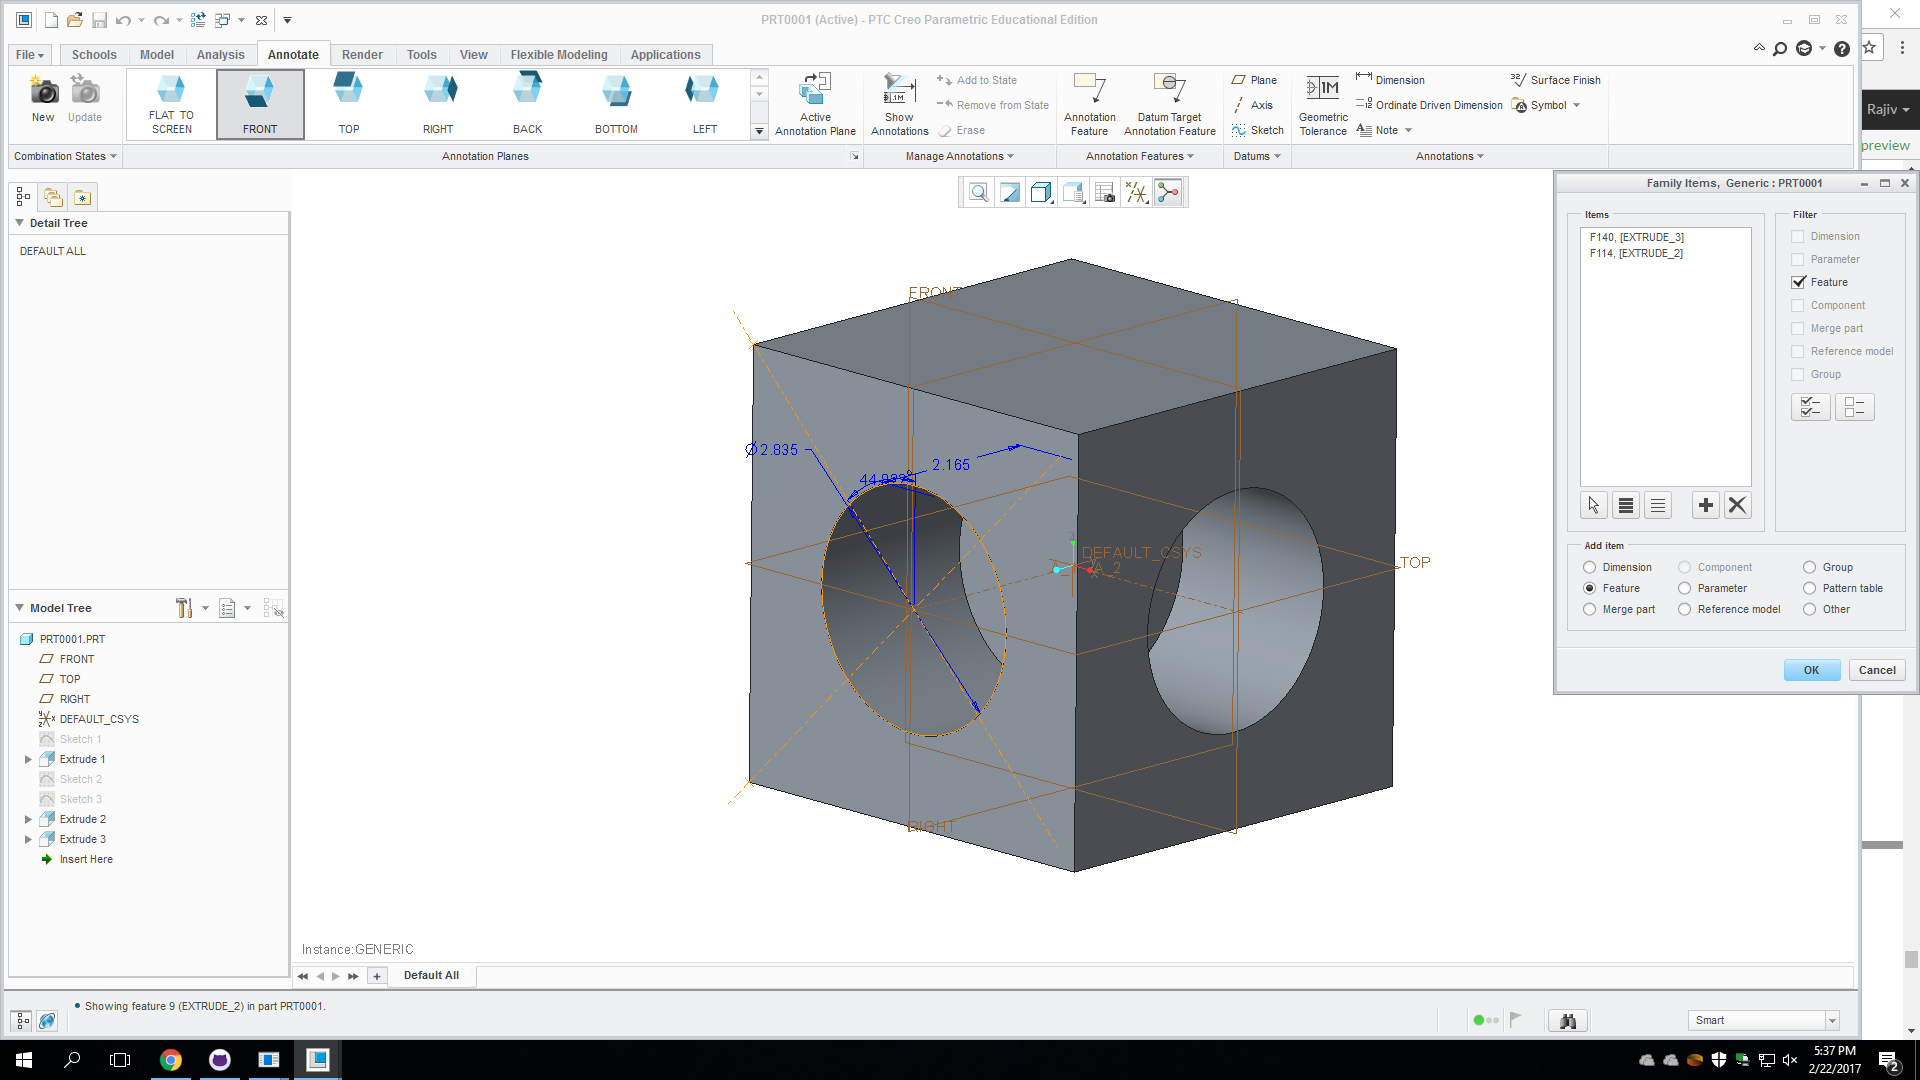
\includegraphics[width=0.7\linewidth]{CAD/Technique/FamilyTableFolder/Capture11.png}
  \caption{Settings customization window.}
  \label{fig:Mod_Ins_1}
\end{figure}

\begin{figure}[ht!]
\centering
  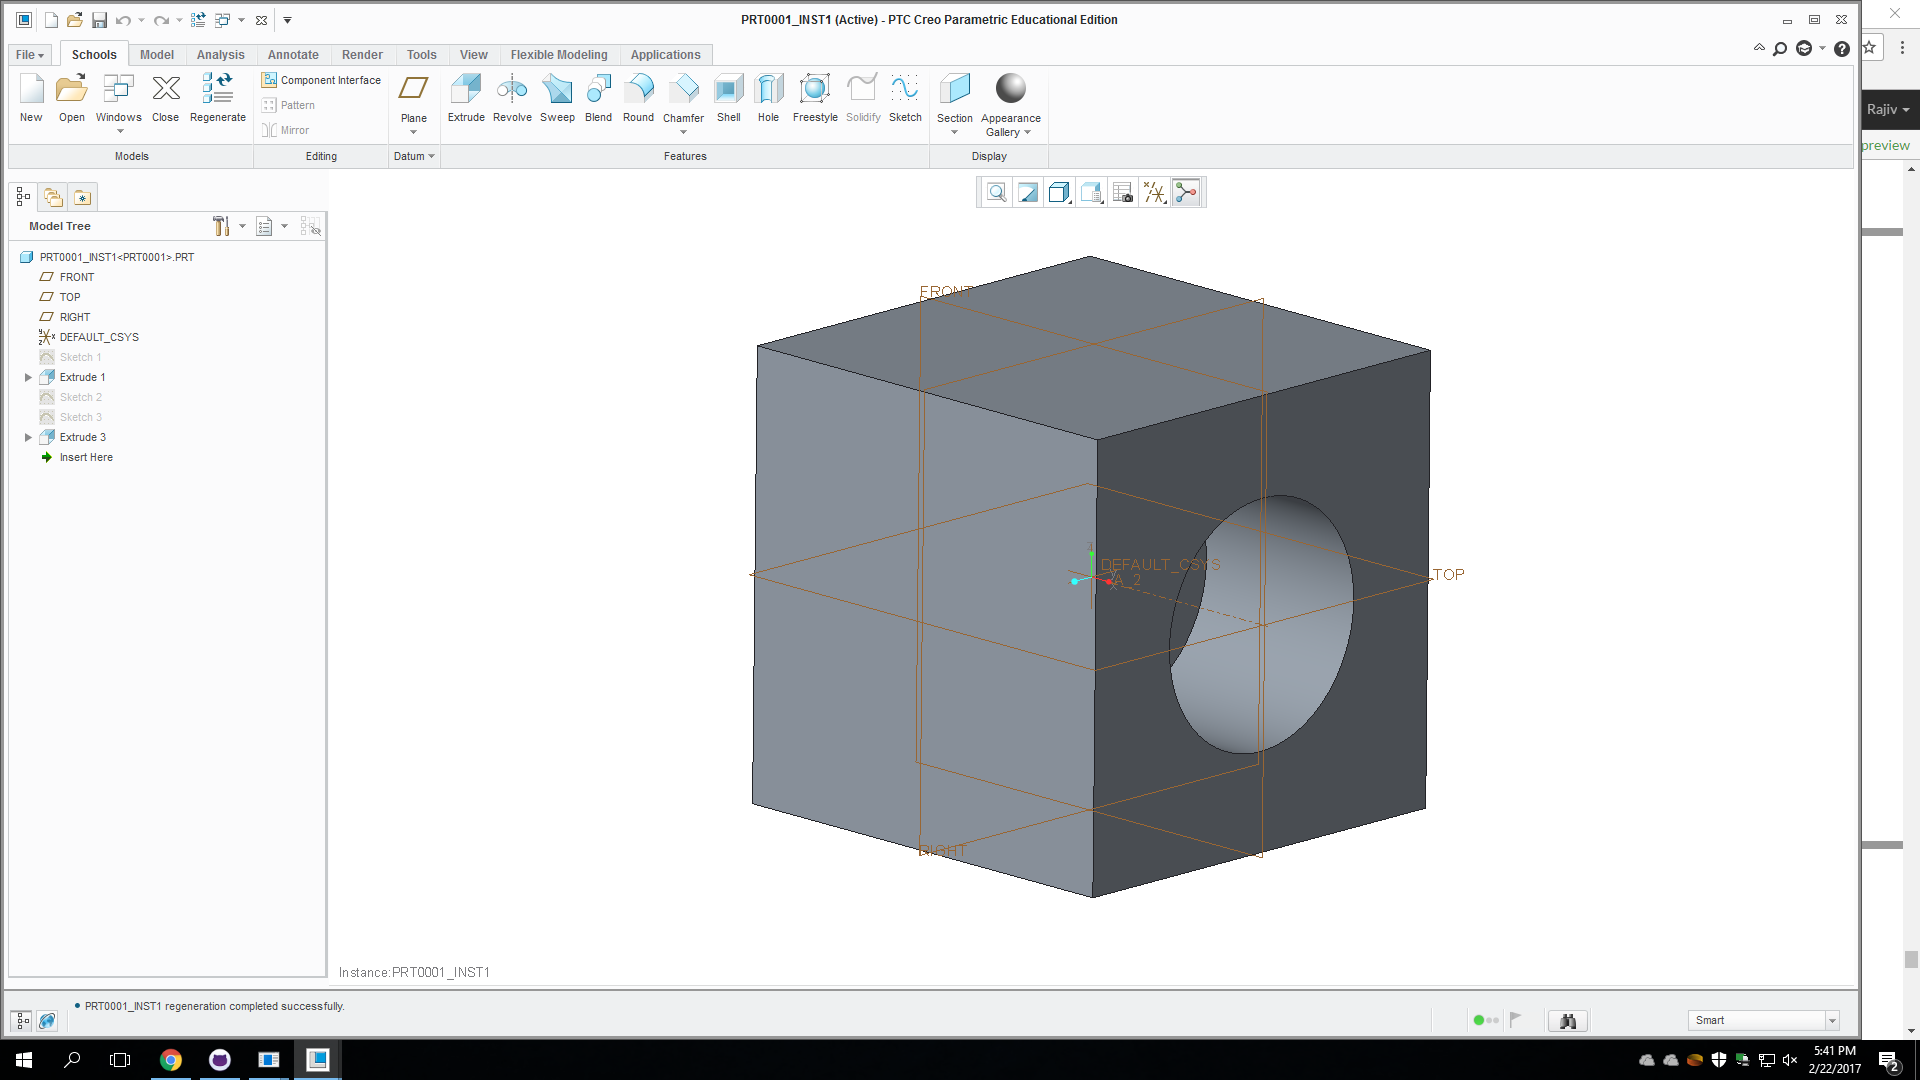
\includegraphics[width=0.7\linewidth]{CAD/Technique/FamilyTableFolder/Capture15.png}
  \caption{Settings customization window.}
  \label{fig:Mod_Ins_2}
\end{figure}

\begin{figure}[ht!]
\centering
  \includegraphics[width=0.7\linewidth]{CAD/Technique/FamilyTableFolder/Capture_16.png}
  \caption{Settings customization window.}
  \label{fig:Mod_Ins_3}
\end{figure}

% \begin{figure}[ht!]
% \centering
%   \includegraphics[width=0.7\linewidth]{Meeting/February/XXX.jpg}
%   \caption{New Triangle Supports}
%   \label{fig:Tri_Sup_Dra}
% \end{figure}

%  ↑ 
